\chapter{Planos}

\section{Plano de ubicación general de la red}

\section{Planos de planta con puntos de red y canalizaciones}

\section{Plano de racks, patch panels y salas de telecomunicaciones}

\section{Plano de backbone}

\section{Detalles constructivos de ductos, bandejas y registros}

Para la implementación física se seguirán las normas \textbf{ANSI/TIA-569-D} :

\begin{itemize}
    \item \textbf{Bandejas portacables}: En los pasillos principales (rutas troncales), se instalarán bandejas tipo escalerilla o bandejas metálicas perforadas de 200x50 mm suspendidas sobre el cielo raso para organizar el backbone y el cableado horizontal.
    
    \item \textbf{Ductería}: Se utilizará \textbf{tubo conduit de PVC de 1 ¼"} para los pases de muros y áreas estratégicas, asegurando un radio de curvatura mínimo para no dañar los cables Cat6A.
    
    \item \textbf{Canaletas}: En interiores de aulas y oficinas, se emplearán canaletas de PVC autoextinguible (tipo 20x12 mm o 40x25 mm) adosadas a la pared para una distribución estética.
    
    \item \textbf{Registros}: Se instalarán cajas de paso de PVC de 150x150x80 mm en cada derivación importante para facilitar el mantenimiento y futuras expansiones.
\end{itemize}

\begin{figure}[H]
    \centering
    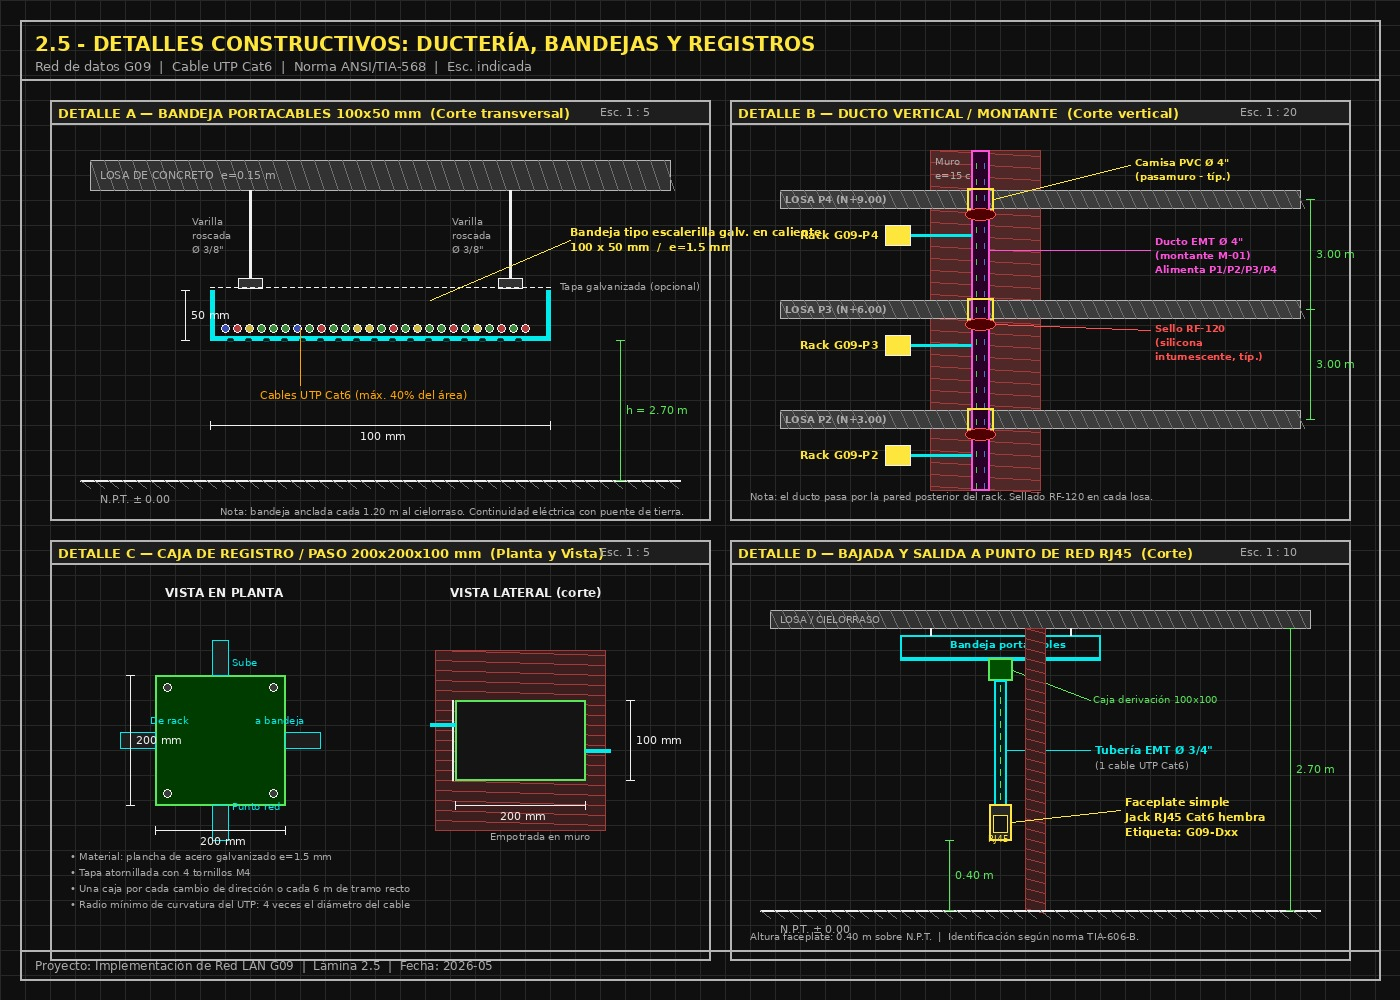
\includegraphics[width=1.0\linewidth]{figures/figuresMarco/detales_constructivos.jpeg}
    \caption{}
    \label{fig:placeholder}
\end{figure}

\section{Diagrama de puesta a tierra}
